\documentclass[12pt,graphicx,caption,rotating]{article}
\textheight=24cm
\textwidth=18cm
\topmargin=-2cm
\oddsidemargin=0cm
\usepackage[utf8x]{inputenc}
\usepackage[activeacute,spanish]{babel}
\usepackage{amssymb,amsfonts}
\usepackage[tbtags]{amsmath}
\usepackage{pict2e}
\usepackage{float}
\usepackage[all]{xy}
\usepackage{graphics,graphicx,color,colortbl}
\usepackage{times}
\usepackage{subfigure}
\usepackage{wrapfig}
\usepackage{multicol}
\usepackage{cite}
\usepackage{url}
\usepackage[tbtags]{amsmath}
\usepackage{amsmath,amssymb,amsfonts,amsbsy}
\usepackage{bm}
\usepackage{algorithm}
\usepackage{algorithmic}
\usepackage[centerlast, small]{caption}
\usepackage[colorlinks=true, citecolor=blue, linkcolor=blue, urlcolor=blue, breaklinks=true]{hyperref}
\hyphenation{ele-men-tos he-rra-mi-en-ta cons-tru-yen trans-fe-ren-ci-a pro-pu-es-tas si-mu-lar vi-sua-li-za-cion}

\begin{document}
\title{\textbf{\huge{Segundo Parcial de Electrónica de Potencia.}}}
\author{David Ricardo Martínez Hernández \textbf{Código:} 261931\\
	\href{}{drmartinezhe@unal.edu.co}\\
	Universidad Nacional de Colombia}
\date{}
\maketitle

\section{Análisis de Tensión.}
\noindent
\subsection{Tensión de entrada}
\noindent
Las tensiones en la entrada del circuito son:
\begin{equation}
 V_a = V_p \sin \left (\omega t \right)
 \label{ecu1}
\end{equation}
\begin{equation}
 V_b = V_p \sin \left (\omega t - \frac{2 \pi}{3}\right)
 \label{ecu2}
\end{equation}
\begin{equation}
 V_c = V_p \sin \left (\omega t+ \frac{2 \pi}{3}\right )
 \label{ecu3}
\end{equation}

\subsection{Tensión de los arreglos}
\noindent
Como el primer arreglo tiene una configuración estrella – estrella y la relación de transformación es de 1 se tiene que:
\begin{equation}
 V_{a1_{s}} = V_a = V_p \sin \left (\omega t \right)
 \label{ecu4}
\end{equation}
\begin{equation}
 V_{b1_{s}} = V_b = V_p \sin \left (\omega t - \frac{2 \pi}{3}\right)
 \label{ecu5}
\end{equation}
\begin{equation}
 V_{c1_{s}} = V_c = V_p \sin \left (\omega t+ \frac{2 \pi}{3}\right )
 \label{ecu6}
\end{equation}
\noindent
Como el segundo arreglo tiene una configuración delta – estrella y la relación de transformación es de $\sqrt{3}$ se tiene que:
\begin{equation}
 {V_{a{2_s}}} = \frac{1}{{\sqrt 3 }}\left( {{V_a} - {V_b}} \right) = {V_p}\sin \left( {\omega t + \frac{\pi }{6}} \right)
 \label{ecu7}
\end{equation}
\begin{equation}
 {V_{b{2_s}}} = \frac{1}{{\sqrt 3 }}\left( {{V_b} - {V_c}} \right) = {V_p}\sin \left( {\omega t - \frac{{2\pi }}{3} + \frac{\pi }{6}} \right) = {V_p}\sin \left( {\omega t + \frac{{5\pi }}{6}} \right)
 \label{ecu8}
\end{equation}
\begin{equation}
 {V_{c{2_s}}} = \frac{1}{{\sqrt 3 }}\left( {{V_c} - {V_a}} \right) = {V_p}\sin \left( {\omega t + \frac{{2\pi }}{3} + \frac{\pi }{6}} \right) = {V_p}\sin \left( {\omega t + \frac{\pi }{2}} \right)
 \label{ecu9}
\end{equation}
\begin{figure}[H]
	\centering
		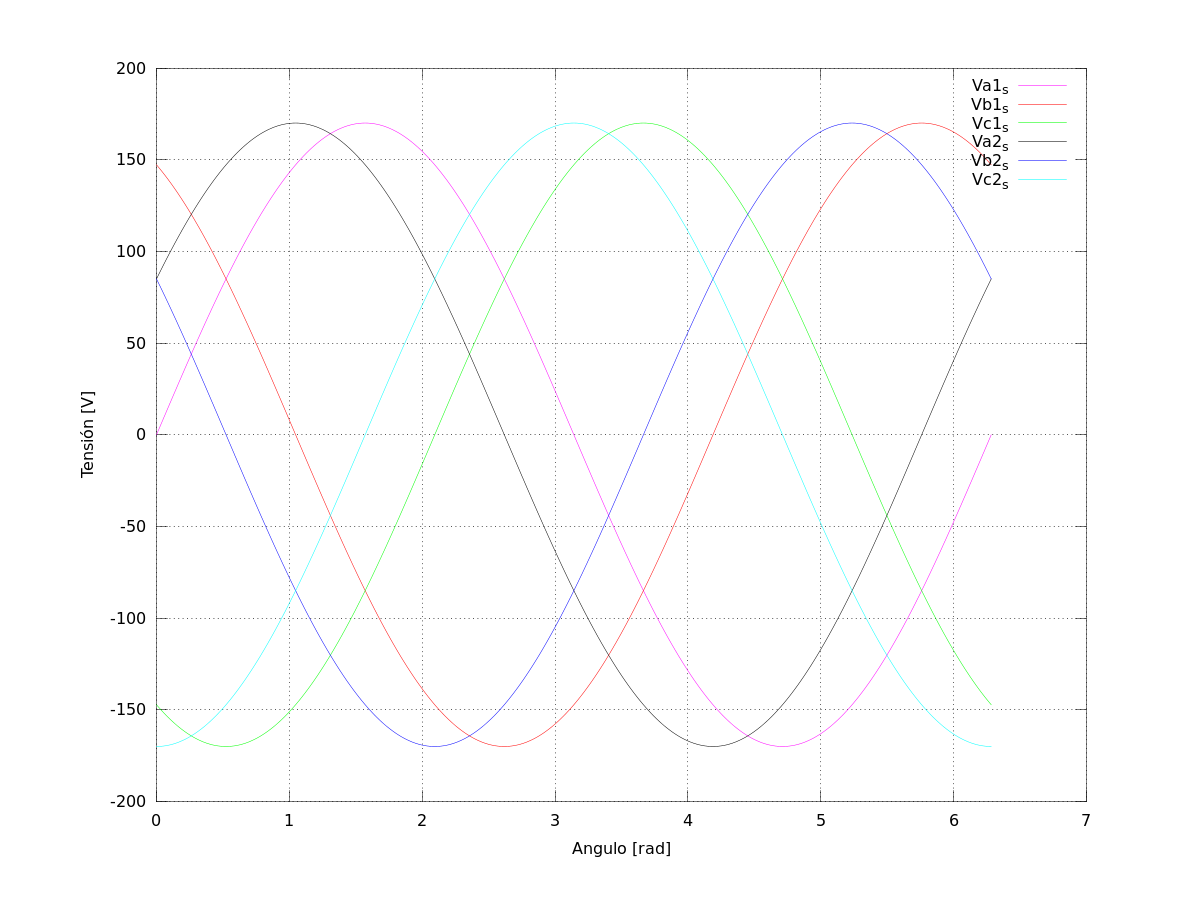
\includegraphics[scale=0.4]{tensiones_in.png}
	\caption{Tensiones de salida de los arreglos Serie, antes de los diodos rectificadores.}
	\label{fig1}
\end{figure}
\noindent
Como el tercer arreglo tiene una configuración estrella – estrella y la relación de transformación es de $1.93185$ se tiene que:
\begin{equation}
 V_{a1_{p}} = 1.93185 V_a = 1.93185  V_p \sin \left (\omega t \right)
 \label{ecu10}
\end{equation}
\begin{equation}
 V_{b1_{s}} = 1.93185  V_b = 1.93185  V_p \sin \left (\omega t - \frac{2 \pi}{3}\right)
 \label{ecu11}
\end{equation}
\begin{equation}
 V_{c1_{s}} = 1.93185  V_c = 1.93185  V_p \sin \left (\omega t+ \frac{2 \pi}{3}\right )
 \label{ecu12}
\end{equation}
\noindent
Como el cuarto arreglo tiene una configuración delta – estrella y la relación de transformación es de $1.93185$ se tiene que:
\begin{equation}
 {V_{a{2_p}}} = \frac{1.93185}{{\sqrt 3 }}\left( {{V_a} - {V_b}} \right) = 1.93185 {V_p}\sin \left( {\omega t + \frac{\pi }{13}} \right)
 \label{ecu13}
\end{equation}
\begin{equation}
 {V_{b{2_p}}} = \frac{1.93185}{{\sqrt 3 }}\left( {{V_b} - {V_c}} \right) = 1.93185 {V_p}\sin \left( {\omega t - \frac{{2\pi }}{3} + \frac{\pi }{6}} \right) = 1.93185 {V_p}\sin \left( {\omega t + \frac{{5\pi }}{6}} \right)
 \label{ecu14}
\end{equation}
\begin{equation}
 {V_{c{2_p}}} = \frac{1.93185}{{\sqrt 3 }}\left( {{V_c} - {V_a}} \right) = 1.93185 {V_p}\sin \left( {\omega t + \frac{{2\pi }}{3} + \frac{\pi }{6}} \right) = 1.93185 {V_p}\sin \left( {\omega t + \frac{\pi }{2}} \right)
 \label{ecu15}
\end{equation}
\begin{figure}[H]
	\centering
		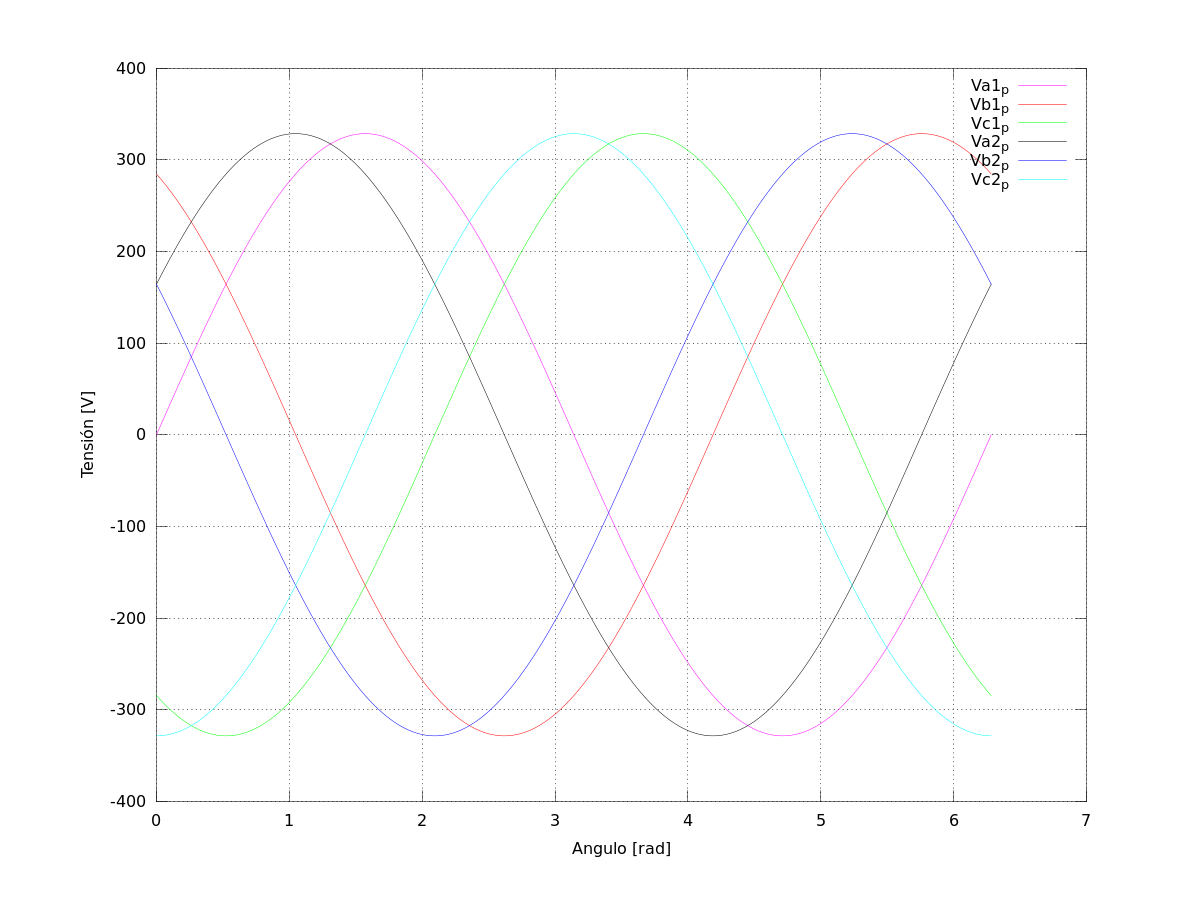
\includegraphics[scale=0.4]{tensiones_in_2.png}
	\caption{Tensiones de salida de los arreglos Paralelo, antes de los diodos rectificadores.}
	\label{fig2}
\end{figure}

\subsubsection{Tensiones después de los diodos}
\noindent
Para determinar las tensiones que se obtienen después de los diodos rectificadores se utilizó la ecu.(\ref{ecu16}) como se muestra en la Figura.~\ref{fig3}:
\begin{equation}
 V_{out_s} = Max (V_{a1_s}, V_{b1_s}, V_{c1_s})- Min (V_{a1_s}, V_{b1_s}, V_{c1_s}) + Max (V_{a2_s}, V_{b2_s}, V_{c2_s})- Min (V_{a2_s}, V_{b2_s}, V_{c2_s}) 
\label{ecu16}
\end{equation}
\begin{figure}[H]
	\centering
		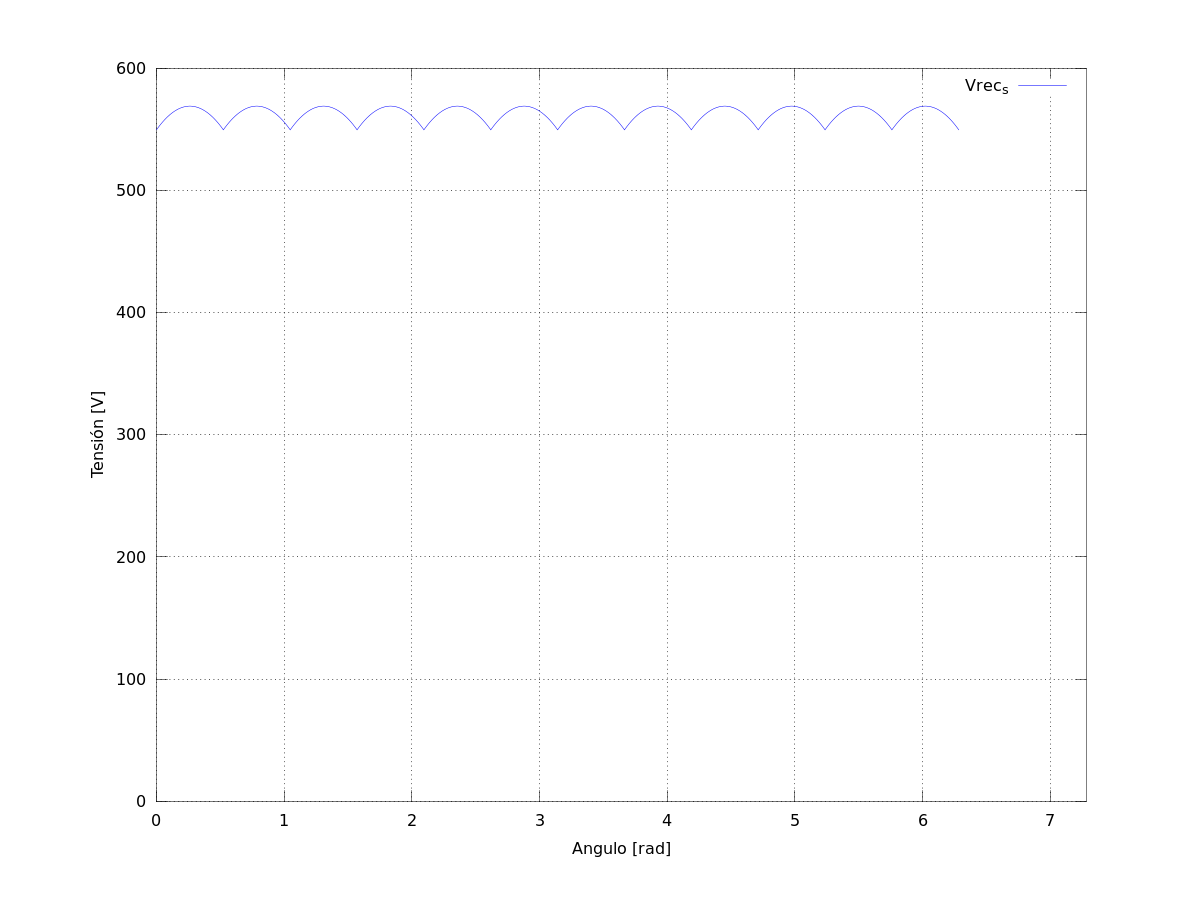
\includegraphics[scale=0.3]{ten_rec_s.png}
	\caption{Tensiones de salida de los diodos para los arreglos Serie.}
	\label{fig3}
\end{figure}
\noindent
Al colocar ambos circuitos en paralelo solo dos de los doce diodos se encontrarán activos al mismo tiempo teniendo en cuenta las diferencias entre las tensiones linea a linea como se observa en la Figura.~\ref{fig4}.
\begin{figure}[H]
	\centering
		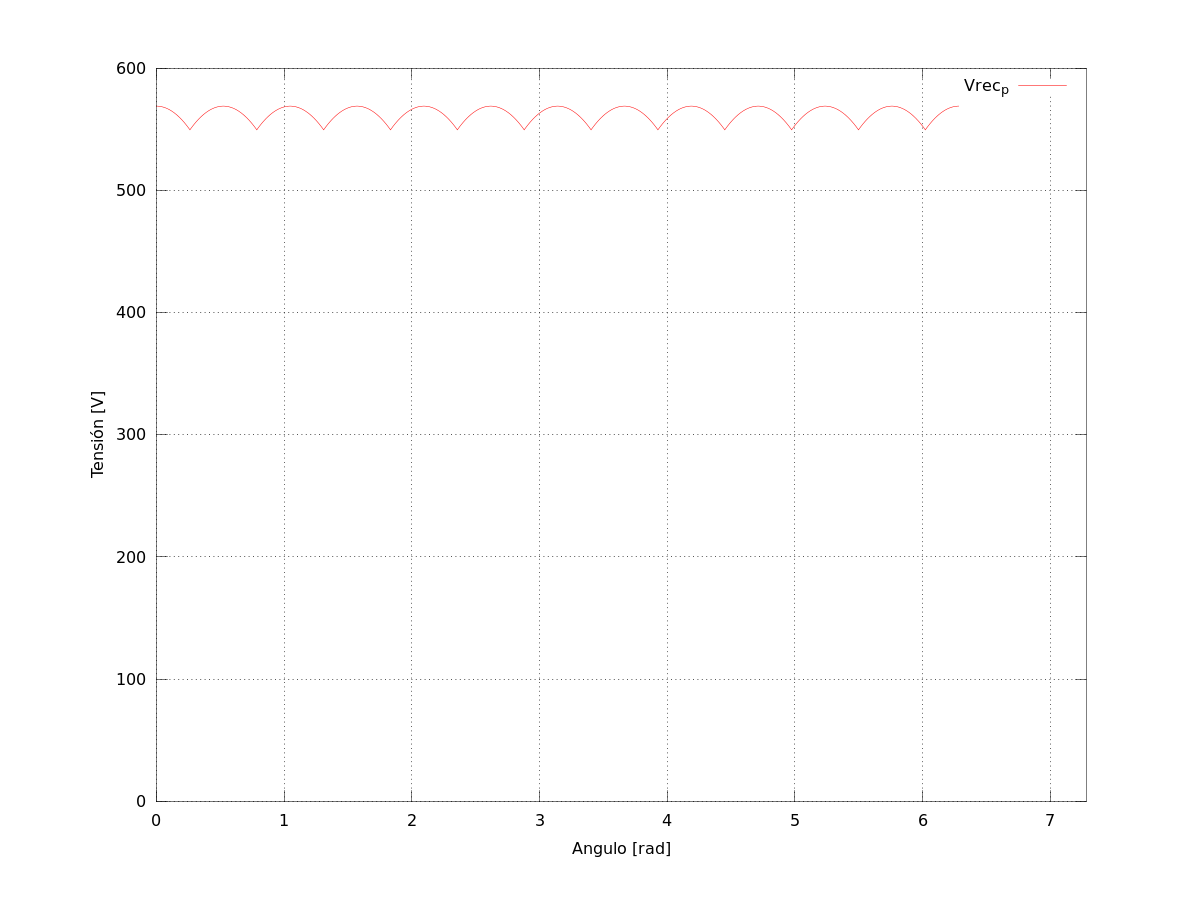
\includegraphics[scale=0.3]{ten_rec_p.png}
	\caption{Tensiones de salida de los diodos para los arreglos Paralelo.}
	\label{fig4}
\end{figure}

\subsection{Tensión de salida en la fuente de corriente}
\noindent
La tensión de salida en la fuente de corriente es la suma de la ecu.(\ref{ecu17}) mostrado en la Figura.~\ref{fig5}:
\begin{equation}
 V_{out} = V_{out_s} + V_{out_p}
 \label{ecu17}
\end{equation}
\begin{figure}[H]
	\centering
		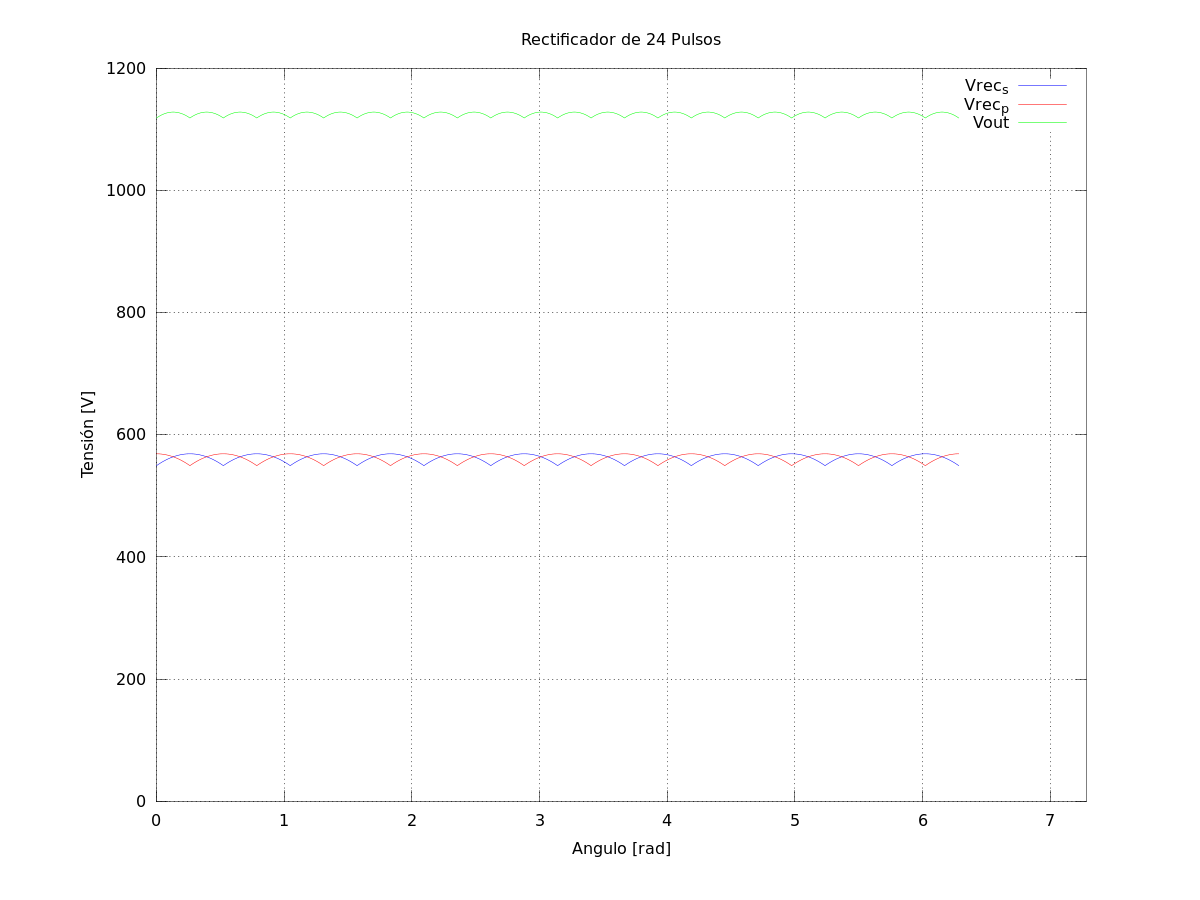
\includegraphics[scale=0.3]{ten_rec.png}
	\caption{Tensiones de salida de los diodos para los arreglos y tensión en la fuente de corriente.}
	\label{fig5}
\end{figure}
\noindent
La tensión promedio se determina por medio de la ecu.(\ref{ecu18}), dando como resultado $\overline {{V_{out}}} \approx 1124.7 [V]$.
\begin{equation}
 \overline {{V_{out}}}  = \overline {{V_{ou{t_s}}}}  + \overline {{V_{ou{t_p}}}}
 \label{ecu18}
\end{equation}

\section{Análisis de Corriente.}

\begin{figure}[H]
	\centering
		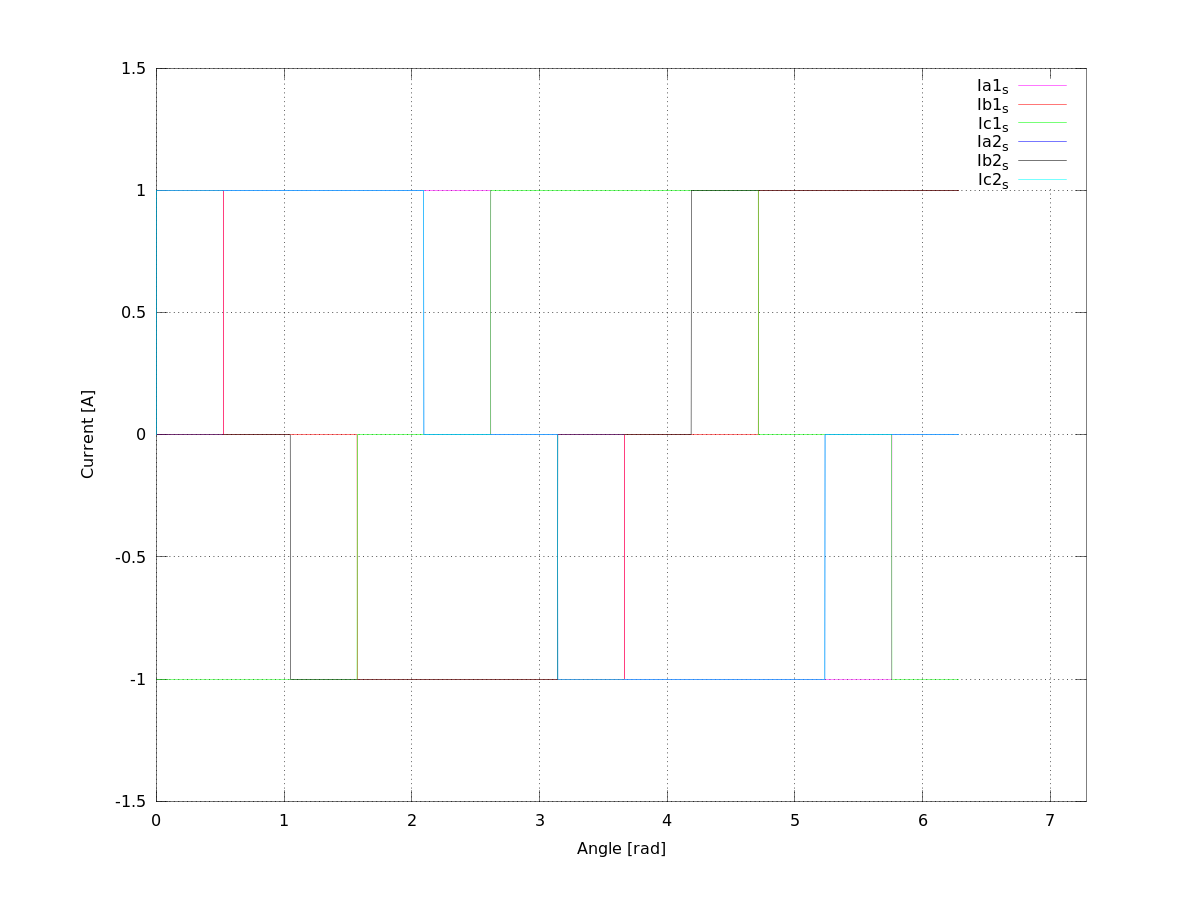
\includegraphics[scale=0.3]{corr_s.png}
	\caption{Salida de corriente para el arreglo en serie.}
	\label{fig6}
\end{figure}
\noindent
\begin{figure}[H]
	\centering
		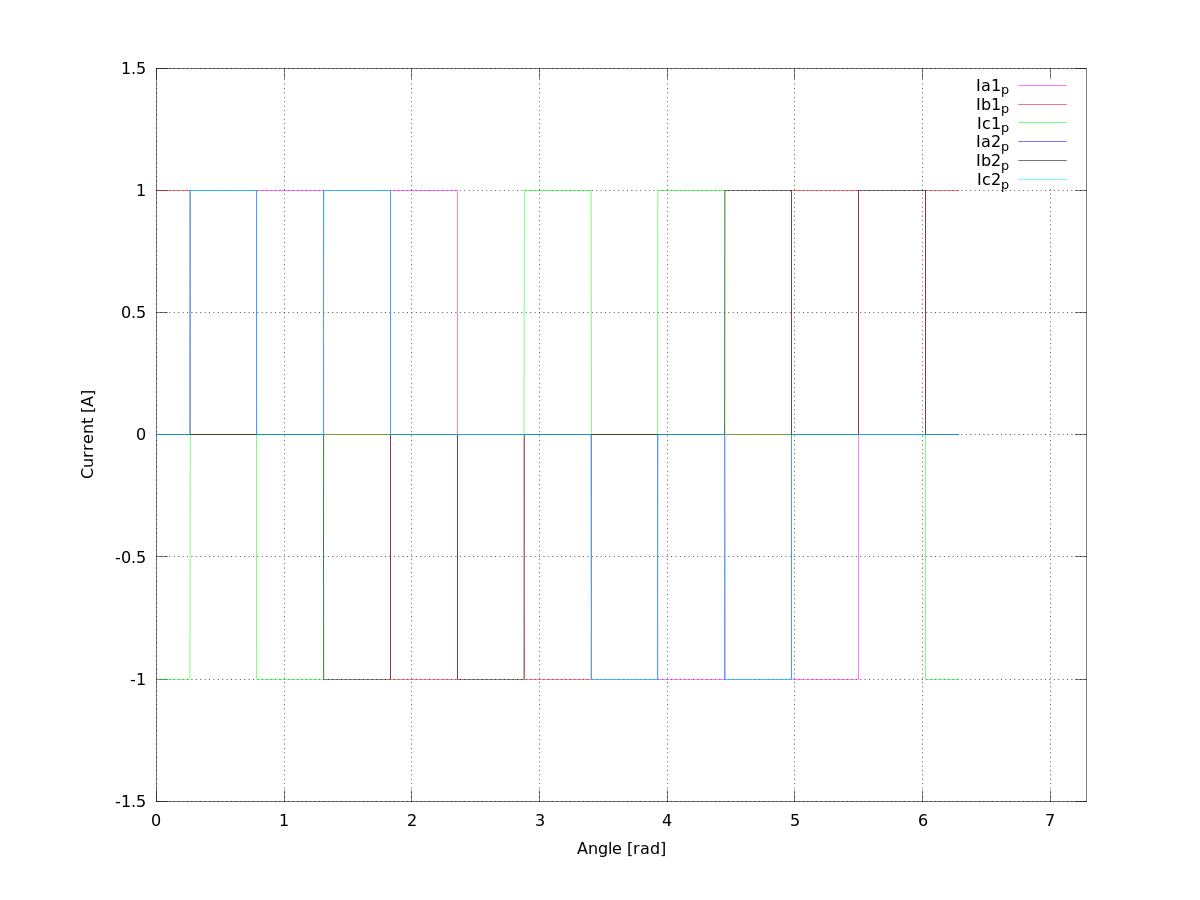
\includegraphics[scale=0.3]{corr_p.png}
	\caption{Salida de corriente para el arreglo en paralelo.}
	\label{fig7}
\end{figure}
\noindent
Para determinar la corriente de entrada para la fase $A$ se utilizaron las siguiente ecuaciones:
\begin{equation}
 I_{a_1} = I_{a1_s}
 \label{ecu19}
\end{equation}
\begin{equation}
 I_{a_2}=\frac{I_{a2_s}-I_{b2_s}}{\sqrt{3}}
 \label{ecu20}
\end{equation}
\begin{equation}
 I_{a_3}=I_{a1_p}*1.93185;
 \label{ecu21}
\end{equation}
\begin{equation}
 I_{a_4}=1.93185\frac{I_{a2_p}-I_{b2_p}}{\sqrt{3}}
 \label{ecu22}
\end{equation}
\noindent
El resultado de las gráficas de las corrientes de entrada para cada fase se encuentran en la Figura.~\ref{fig8}.
\begin{figure}[H]
	\centering
		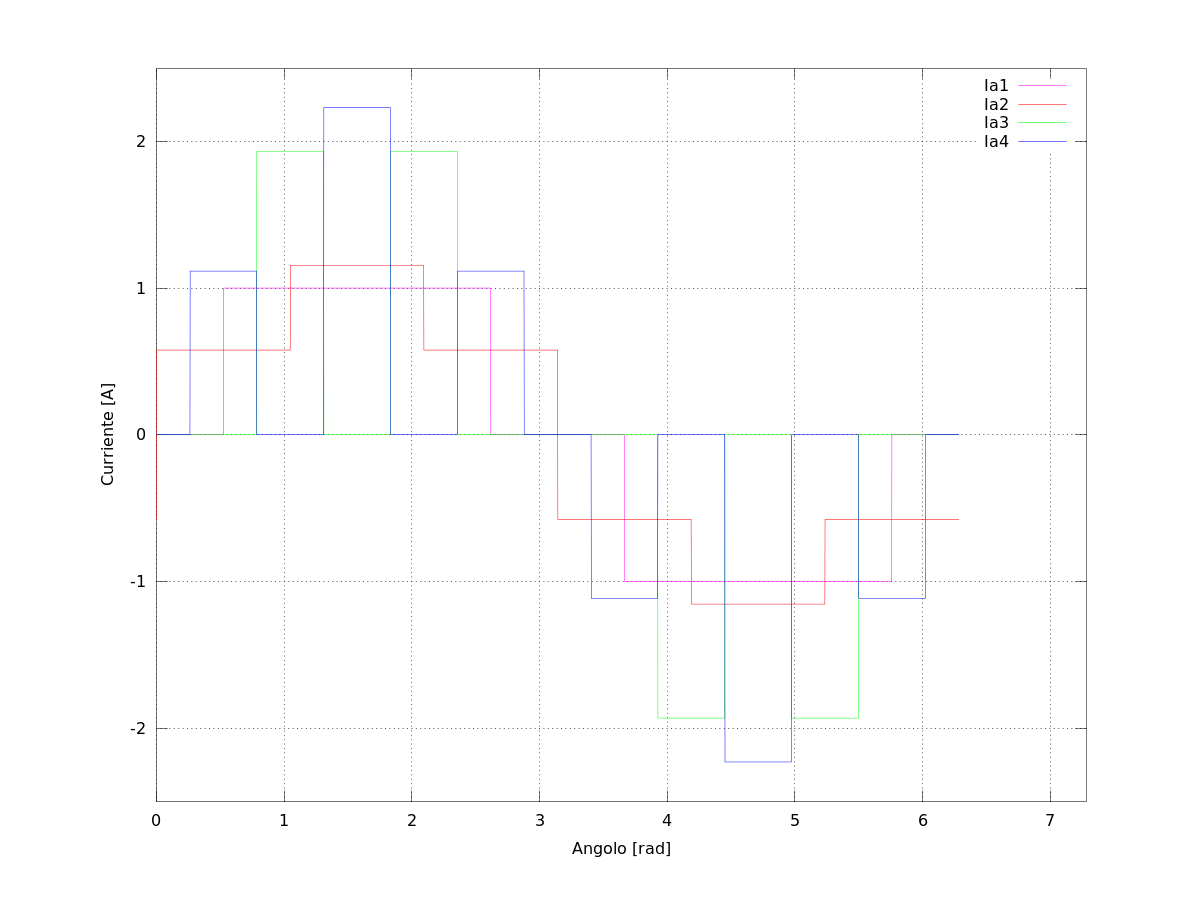
\includegraphics[scale=0.3]{corr_sal.png}
	\caption{Corrientes de entrada para cada fase.}
	\label{fig8}
\end{figure}
\begin{equation}
 I_{a} = I_{a_1} + I_{a_2} + I_{a_3} + I_{a_4}
 \label{ecu23}
\end{equation}
\noindent
El resultado de la corriente de entrada para la fase $A$ se encuentran en la Figura.~\ref{fig9}.
\begin{figure}[H]
	\centering
		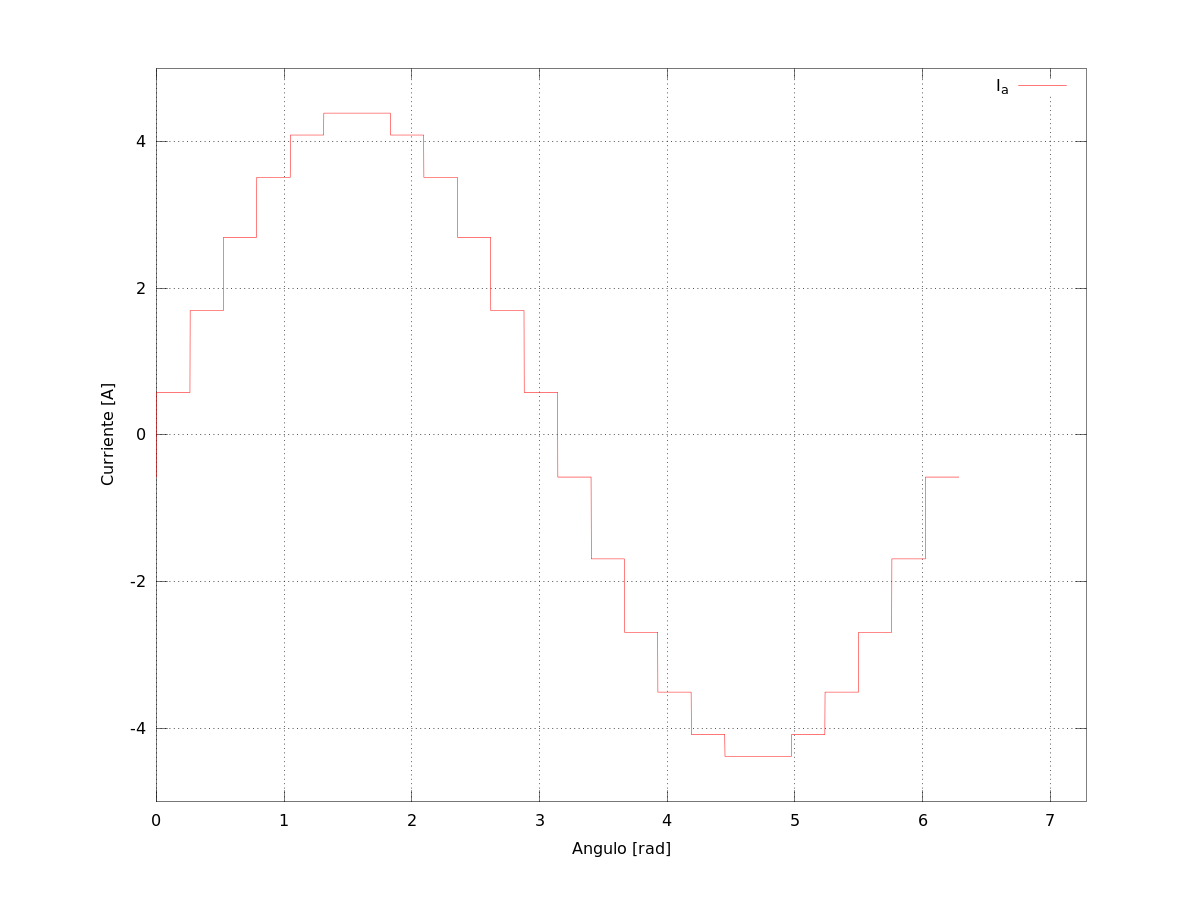
\includegraphics[scale=0.4]{corr_sal_f.png}
	\caption{Corriente de entrada para la fase $A$.}
	\label{fig9}
\end{figure}
\noindent
La corriente RMS de entrada se determino por medio de la ecu.(\ref{ecu24}), dando como resultado $I_{out_{RMS}} \approx 3.127 [A] $.
\begin{equation}
 {I_{{a_{RMS}}}} = \sqrt {\frac{2}{\pi }\left( {{{\int\limits_0^{{\raise0.7ex\hbox{$\pi $} \!\mathord{\left/
 {\vphantom {\pi  {12}}}\right.\kern-\nulldelimiterspace}
\!\lower0.7ex\hbox{${12}$}}} {\left( {\frac{1}{{\sqrt 3 }}} \right)} }^2}d\left( {\omega t} \right) + {{\int\limits_{{\raise0.7ex\hbox{$\pi $} \!\mathord{\left/
 {\vphantom {\pi  {12}}}\right.\kern-\nulldelimiterspace}
\!\lower0.7ex\hbox{${12}$}}}^{{\raise0.7ex\hbox{$\pi $} \!\mathord{\left/
 {\vphantom {\pi  6}}\right.\kern-\nulldelimiterspace}
\!\lower0.7ex\hbox{$6$}}} {\left( {1.6927} \right)} }^2}d\left( {\omega t} \right) + {{\int\limits_{{\raise0.7ex\hbox{$\pi $} \!\mathord{\left/
 {\vphantom {\pi  6}}\right.\kern-\nulldelimiterspace}
\!\lower0.7ex\hbox{$6$}}}^{{\raise0.7ex\hbox{$\pi $} \!\mathord{\left/
 {\vphantom {\pi  4}}\right.\kern-\nulldelimiterspace}
\!\lower0.7ex\hbox{$4$}}} {\left( {\frac{1}{{\sqrt 3 }}} \right)} }^2}d\left( {\omega t} \right) + {{\int\limits_{{\raise0.7ex\hbox{$\pi $} \!\mathord{\left/
 {\vphantom {\pi  4}}\right.\kern-\nulldelimiterspace}
\!\lower0.7ex\hbox{$4$}}}^{{\raise0.7ex\hbox{$\pi $} \!\mathord{\left/
 {\vphantom {\pi  3}}\right.\kern-\nulldelimiterspace}
\!\lower0.7ex\hbox{$3$}}} {\left( {1.6927} \right)} }^2}d\left( {\omega t} \right)} \right)}
 \label{ecu24}
\end{equation}

\section{Análisis de Potencia.}
\noindent
La potencia activa de la fuente de corriente se determino por medio de la ecu.(\ref{ecu25}), dando como resultado $P_{out} \approx 1124.7 [W]$.
\begin{equation}
 P_{out} = \overline {{V_{out}}} \overline {{I_{out}}}
 \label{ecu25}
\end{equation}
\noindent
La potencia aparente en la fase $A$ se determino por medio de la ecu.(\ref{ecu26}), dando como resultado $S_A \approx 375.89 [VA]$.
\begin{equation}
 S_A = V_{a_{RMS}} I_{a_{RMS}}
\label{ecu26} 
\end{equation}
\noindent
La potencia activa en la fase $A$ se determino por medio de la ecu.(\ref{ecu27}), dando como resultado $P_{a_A} \approx 374.9 [W]$.
\begin{equation}
 P_{a_A} = \frac{P_{out}}{3}
 \label{ecu27}
\end{equation}
\noindent
El factor de potencia se determino por medio de la ecu.(\ref{ecu28}), dando como resultado $PF \approx 0.99737$.
\begin{equation}
 PF=\frac{P_{a_A}}{S_A}
 \label{ecu28}
\end{equation}

\section{Distorsión Armónica.}
\noindent
La distorsión armónica se determino por medio de la ecu.(\ref{ecu29}), dando como resultado $THD \approx 0.072712$.
\begin{equation}
 THD = \sqrt{\left (\frac{1}{PF}\right )^2 -1}
 \label{ecu29}
\end{equation}


\end{document}